\subsection{Integracja konturów w pierwszorzędowej korze wzrokowej}
\label{integracjaLi}

%LI - 37
%%%Receptors can be classified broadly as excitatory (causing an increase in firing rate), inhibitory (causing a decrease in firing rate), or modulatory (causing long-lasting effects not directly related to firing rate).

Aby zaczerpnąć z prezentowanych wcześniej technik \ref{integracjaSEC} oraz \ref{hypercolumn} został stworzony inny model ekstrakcji i integracji konturów.\\ 
\begin{figure}[ht]
	\centering
	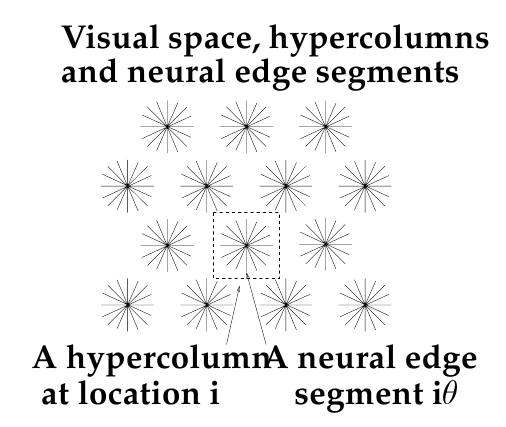
\includegraphics[width=0.55\textwidth]{images/li_hypercolumn.png}
	\caption{Przestrzeń hiperkolumn w modelu integracji konturów \cite{Li1998}.}
	\label{fig:li_hypercolumn}
\end{figure}

\begin{figure}[ht]
	\centering
	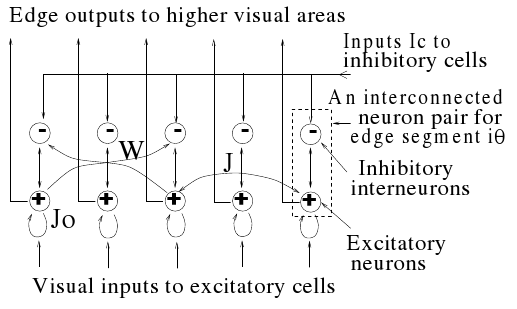
\includegraphics[width=0.7\textwidth]{images/li_arch.png}
	\caption{Architektura częściowa sieci prezentującej podstawowe elementy składowe modelu z pracy \cite{Li1998}.}
	\label{fig:li_arch}
\end{figure}

Podstawowym elementem modelu integracji konturów jest hiperkolumna -- która zgodnie z tym co zostało zaobserwowane w korze wzrokowej kota -- jest ona umieszczona w heksagonalnej przestrzeni, co znaczy, że każda z nich 6 sąsiadujących. Składa się ona z segmentów krawędziowych\footnote{Tłumaczenie z języka angielskiego -- edge segment.}, a każdy segment może zostać określony numerem kolumny $i$ w przypadku jeśli wszystkie są ponumerowane oraz kątem $\theta$ który odpowiada za nachylenie krawędzi w segmencie. W każdym segmencie znajduje się para neuronów, inhibitor i ekscytator, które są ze sobą połączone. Gdy w części obrazu objętej obszarem $i$ znajduje się krawędź zorientowana pod kątem $\beta$ oraz siłą/intensywnością $\hat{I}_{i\beta}$ (rysunek \ref{fig:li_hypercolumn}), wtedy segment otrzymuje na wejście sygnał $I_{i\beta}$ który można wyliczyć z poniższego wzoru. 
$$I_{i\beta} = \hat{I}_{i\beta} \phi (\theta - \beta)$$ 
gdzie 
$$\phi(\theta - \beta) = e^{-|\theta - \beta| / (\phi / 8 )}$$
jest pewną funkcją odchylenia. Rzecz jasna segmenty poza hiperkolumną nie dostają żadnego sygnału.\\
Określa się też parametr nazywany barierą membranową oznaczaną $x_{i\theta}$ dla ekscytatora oraz $y_{i\theta}$ dla inhibitora oraz funkcje wyjścia dla każdego z neuronów $g_x(x_{i\theta})$ oraz $g_y(y_{i\theta})$.\\
Architektura tej sieci jest zaprezentowana na rysunku \ref{fig:li_arch}.\\

\begin{figure}[ht]
	\centering
	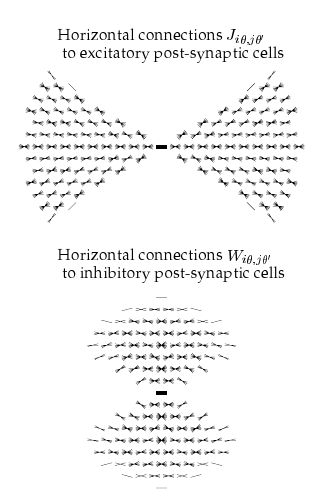
\includegraphics[width=0.45\textwidth]{images/li_field.png}
	\caption{Pole mające wpływ na konkretny jeden segment, w zależności od funkcji odległości $J_{i\theta, j\theta'}$ oraz $W_{i\theta, j\theta'}$ \cite{Li1998}.}
	\label{fig:li_rf}
\end{figure}

Wyniki działania modelu -- wprawdzie skąpe, są przedstawione na rysunku \ref{fig:li_out}.\\

\begin{figure}[ht]
	\centering
	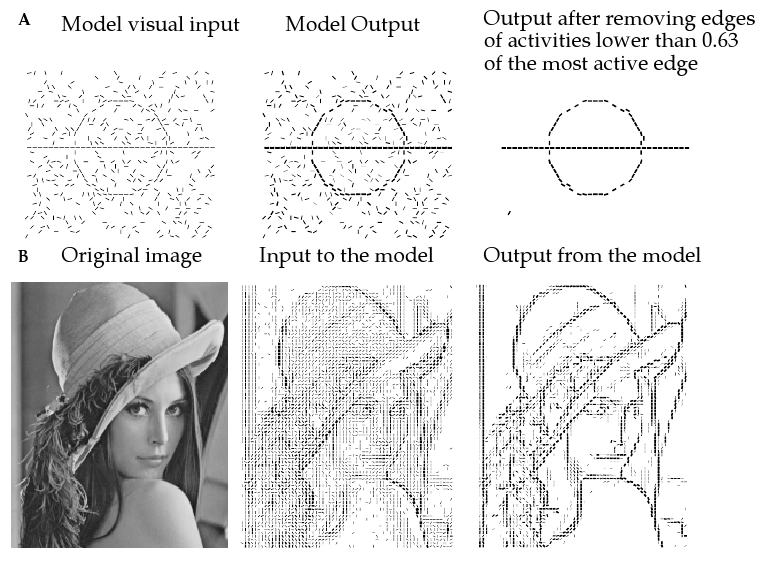
\includegraphics[width=1.00\textwidth]{images/li_out.png}
	\caption{Wyniki działania opisanego wcześniej algorytmu. Praca przedstawia zdjęcie najczęściej poddawane obróbce cyfrowej -- Lenę. Wyraźnie widać, że krawędzie zostały odzyskane w praktycznie doskonały sposób \cite{Li1998}.}
	\label{fig:li_out}
\end{figure}

Autor cytowanej pracy zwraca uwagę na połączenia między-segmentowe. Wyraźnie widać je na schemacie prezentującym architekturę sieci. Co jest istotne, są one realizowane jedynie na 2 sposoby: między ekscytatorami różnych segmentów oraz między ekscytatorem i inhibitorem z różnych segmentów. Nie ma połączeń między inhibitorami, nawet na siebie.\\

Sens sieci jest taki, aby ona się omiatała przez jakiś czas i ustalała swój stan. Konieczne jest bowiem propagowanie wyników -- sygnałów wyjściowych po raz kolejny do wejść neuronów oraz przeliczanie od nowa. Bardzo dobrze jest to przedstawione na rysunku \ref{fig:li_arch}.\\
Aby jednak móc lepiej zaprezentować działanie całości potrzeba trochę formalizmów, których w pracy \cite{Li1998} nie brakuje. 
\begin{align}\label{eqn:li_wzor1}
\dot{x}_{i\theta} = - \alpha_xx_{i\theta} - \sum_{\Delta\theta}\psi(\Delta\theta)g_y(y_{i\theta+\Delta\theta})+ \notag\\
+ J_0g_x(x_{i\theta}) + \sum_{j \neq i, \theta'} J_{i\theta, j\theta'}g_x(x_{j\theta'}) + I_{i\theta} + I_0
\end{align}
\begin{align}\label{eqn:li_wzor2}
\dot{y}_{i\theta} = - \alpha_yy_{i\theta} - g_x(x_{i\theta}) + \sum_{j \neq i, \theta'} W_{i\theta, j\theta'}g_x(x_{j\theta'}) + I_c
\end{align}
Wzory \ref{eqn:li_wzor1} oraz \ref{eqn:li_wzor2} prezentują wyjściowe stany w tak zwanym momencie '$t+1$'. Występujące we wzorach $J_{i\theta, j\theta'}$ oraz $W_{i\theta, j\theta'}$ są w pewnym sensie funkcjami odległości $j\theta'$ od $i\theta$. Funkcje te są pewnej nieprzystępnej postaci -- wyznaczonej doświadczalnie i nie będą tutaj umieszczane, konieczne jest jednak pokazanie sensu tych funkcji. Można go zaprezentować określając pole, jakie ma znaczenie biorąc pod uwagę wpływ sąsiednich pól, na jedno -- konkretne. Przedstawione ono jest na rysunku \ref{fig:li_rf}.\\


Omawiając to podejście należy wspomnieć o uwagach autorki publikacji \cite{Li1998} z której zostały zaczerpnięte przykłady. We wstępie swojej pracy zwraca Ona uwagę na problematykę etapu ekstrakcji konturów z obrazu. Wymienia kilka różnych algorytmów, na które mają związek z tym, jak kontury odzyskiwane są w korze wzrokowej. Zwraca uwagę jednak na to, że nawet bez ograniczeń wynikających z zastosowania podejścia wzorowanego na pierwszorzędowej korze wzrokowej jest to zagadnienie trudne. Wspominany w części \ref{integracjaSEC} algorytm na proste i skuteczne odzyskiwanie krawędzi z obrazu, wprawdzie nie był zastosowany w opisywanej pracy, ale inne algorytmy tego pokroju były przez autorkę testowane. Odnosi się bowiem Ona do nich jako do algorytmów mających problem. Najczęściej wynika on z występowania parametrów, które wymagają dostrojenia przez użytkownika, przez co do dobrej symulacji ekstrakcji konturów nie mogą być zastosowane.\\

Autorka stawia nawet pytanie, czy jest to osiągalne za pomocą modelowania obszaru V1 mózgu, czy może to wymagać wpływu wyższych warstw kory wzrokowej. Opisywane wcześniej biologiczne podstawy funkcjonowania kory wzrokowej wskazują, że może to być bardzo prawdopodobne.
